%! TEX root = diss.tex
\documentclass[../diss.tex]{subfiles}
\chapter{Evaluation}

\section{Evaluation metrics}

Nothing in this section

\section{Parallel matrix-multiplication}

\newpage
See \autoref{fig:example1} for some example plots. There is also
\autoref{fig:example3} which shows some stuff.


% Example figure
\begin{figure}
    \begin{center}
        % \includegraphics[scale=1]{figs/plots/example1.pdf}
        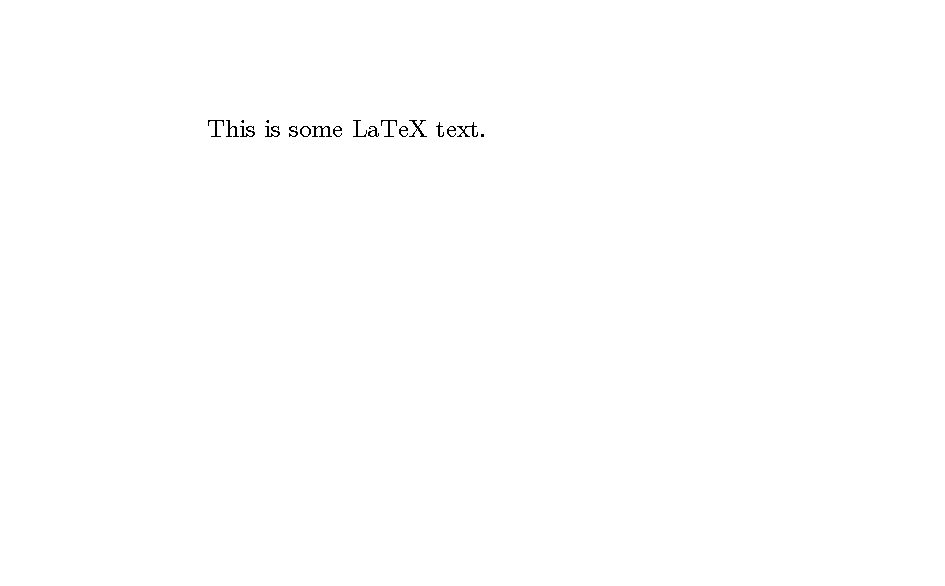
\includegraphics{inkscape-diagrams/template-diagram2.pdf}
    \end{center}
    \caption{Example diagram produced with inkscape}
    \label{fig:example1}
\end{figure}

% Comparison of computation ratio
\begin{figure}%
    \hfill
    \subfigure[Sandy bridge]{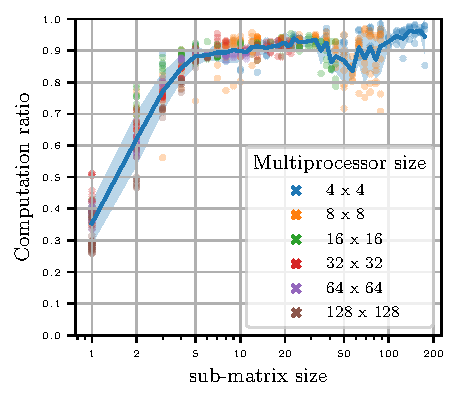
\includegraphics[scale=0.95]{figs/plots/ratio-bucket-sandy-half-scale.pdf}}
    \hfill
    \subfigure[Taihu light]{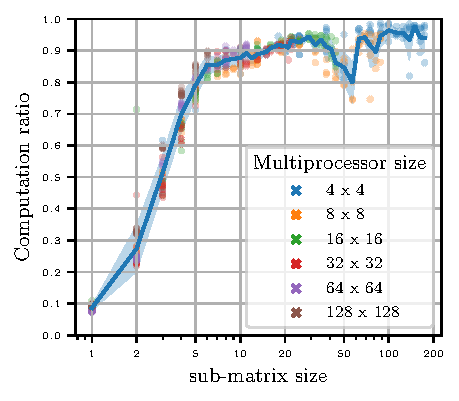
\includegraphics[scale=0.95]{figs/plots/ratio-bucket-taihu-half-scale.pdf}}
    \hfill
    \caption{Title for both, and explain some more...}
    \label{fig:example2}
\end{figure}

% Third example figure
\begin{figure}
    \begin{center}
        % \includegraphics[scale=1]{figs/plots/example3.pdf}
        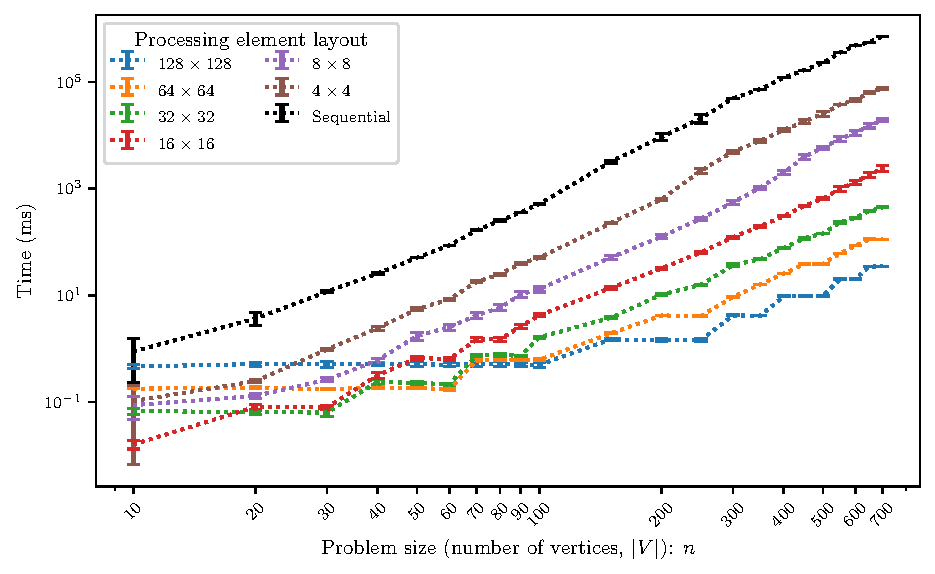
\includegraphics{figs/plots/total-time-scaling-sandy-full-width.pdf}
    \end{center}
    \caption{Sandy bridge total time scaling}
    \label{fig:example3}
\end{figure}

% Fourth example figure
\begin{figure}
    \begin{center}
        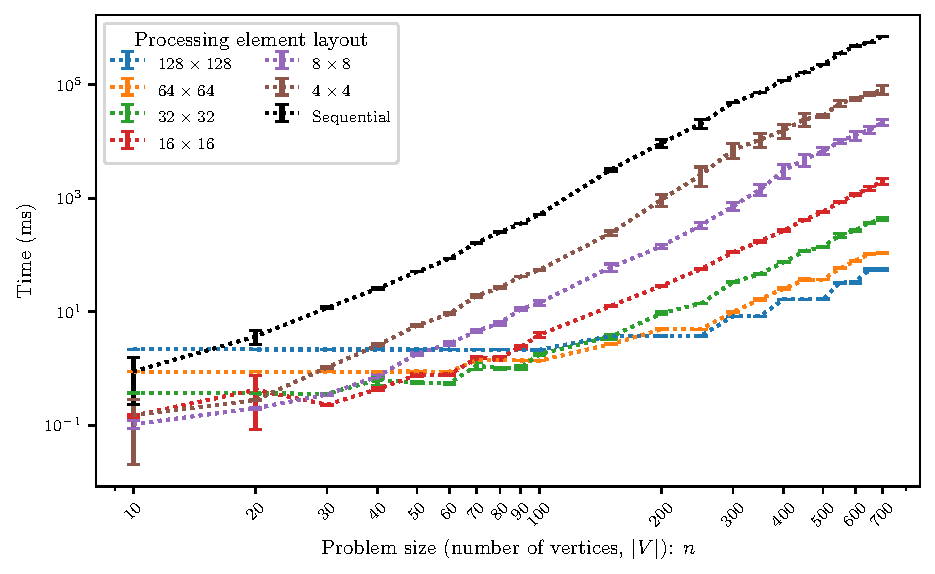
\includegraphics[scale=1]{figs/plots/total-time-scaling-taihu-full-width.pdf}
    \end{center}
    \caption{Taihu light total time scaling}
    \label{fig:example4}
\end{figure}
